\documentclass[12pt]{article}
\usepackage{fullpage}
\usepackage{amsmath}
\usepackage{hyperref}
\usepackage{graphicx}
\usepackage{listings}
\usepackage{float}

\floatstyle{plain}
\newfloat{snippet}{thb}{lop}
\floatname{snippet}{Snippet}


\begin{document}
  \begin{center}
    \textbf{\large Superscalar SMIPS} \\
    6.375 Final Project Proposal\\
    30 March 2011 \\
    
    \vspace{\baselineskip}
    
    \emph{Team}: David S. Greenberg and Bhaskar Mookerji
  \end{center}


%\section{Proposal}


\section{Tomasulo's Algorithm at a Glance}

Before getting into the details of Tomasulo's algorithm, let's try to understand it at a high level. An instruction set architecture (ISA) has a finite number of places in which
it can store variables. These places are called registers. Tomasulo's algorithm dynamically computes the dependencies between instructions so that instructions that
don't have data dependencies can run in parallel, while only the truly data-dependent instructions are run in sequence. This increases the throughput of the system by exploiting
instruction level parallelism (ILP). Tomasulo's algorithm can be seen as a dynamic hardware implementation of Static Single Assignment, a compiler technique that does
the same dependency calculations in software.

The core idea of Tomasulo's algorithm is that each ISA register has a corresponding physical register. Since instructions are dispatched in order but executed out of order,
we can associate the source operands of the instruction with the physical registers corresponding to the ISA registers used in the instruction. The destination register of
the instruction, however, is written to a new physical register, and the destination ISA register is updated to be linked to the new physical register. That way, every 
register is assigned once and only true dependencies affect execution.

Of course, hardware can't be allocated, and so Tomasulo's algorithm allocates the physical registers from a pool and releases registers back into the pool when there are
no more instructions using them as a source operand. The details of this are explained later.

\section{Problem\label{sec:problem}}
Although an elastic pipelined microprocessor is an improvement over an unpipelined processor, its performance suffers due to pipeline stalls.
There are three classes of stalls, two of which are eliminated by Tomasulo's algorithm.

The first class of stall is a Write-After-Read stall. This is where we see an instruction $A$ which reads from register $r_x$ followed by an instruction
$B$ which writes to the same register $r_x$. Normally, $B$'s execution is blocked by $A$ since they both need to access the same register. If $A$ has
several cycles of latency, then $B$ will be stalled until $A$ completes execution. Tomasulo's algorithm eliminates this false dependency by writing the
result of $B$ to a separate physical register, allowing $B$ to execute in parallel with $A$.

The second class of stall is a Write-After-Write stall. This is where we see an instruction $C$ which writes to a register $r_y$ followed by an instruction
$D$ which writes to the same register $r_y$. Normally, since both instructions need to write to the same ISA register, $D$ would be stalled until $C$ completed;
however, Tomasulo's algorithm allows them to execute in parallel since the instructions would each write to separate physical registers.

The third class of stall is a Read-After-Write stall, or a true data dependency. This is where instruction $E$ writes to register $r_z$, and then instruction $F$
reads from register $r_z$. Tomasulo's algorithm does nothing in this case, because since $F$ needs the result of $E$, it must be stalled until $E$ completes.

Let's look at an example snippet of code to understand an example situation in which Tomasulo's algorithm would help (Snippet~\ref{mulmovadd}).
In this simplified assembly language, the format of an instruction is $op$, $src_1$, $\left[src_2\right]$, $dst$; $src2$ is optional.

\begin{snippet}
\begin{verbatim}
mul r1, r2, r3
mov r3, r4
add r1, r2, r3
\end{verbatim}
\caption{Instruction sequence which would benefit from Tomasulo's algorithm}
\label{mulmovadd}
\end{snippet}

Let's assume that multiplies take 4 clock cycles, moves take 1 clock cycle, and adds take 2 clock cycles. Also, let's assume that fetching an instruction takes 1 clock cycle
and happens in parallel with execution. Then executing these instructions in sequence takes a total of 8 clock cycles--one cycle for the initial fetch, followed by each instruction
executing in sequence (Table~\ref{tab:simpleex1}). Since fetches are pipelined, we only see the fetch latency on the initial instruction. Now, if we are using Tomasulo's algorithm, we'll instead
see a total runtime of 6 clock cycles. To understand why, we can look at this table \ref{tab:tomasuloex1}.

\begin{table}
\begin{tabular}{l || c | c | c | c | c | c | c | c}
Cycle & 1 & 2 & 3 & 4 & 5 & 6  & 7 & 8 \\ \hline
Multiply & fetch & exec 1 & exec 2 & exec 3 & exec 4 & & \\
Move & & fetch & stall & stall & stall & exec & \\
Add & & & fetch & stall & stall & stall & exec 1 & exec 2 \\
\end {tabular}
\caption{Snippet \ref{mulmovadd} executed on a simply pipelined microprocessor}
\label{tab:simpleex1}
\end{table}

\begin{table}
\begin{tabular}{l || c | c | c | c | c | c}
Cycle & 1 & 2 & 3 & 4 & 5 & 6 \\ \hline
Multiply & fetch & exec 1 & exec 2 & exec 3 & exec 4 & \\
Move & & fetch & stall & stall & stall & exec \\
Add & & & fetch & exec 1 & exec 2 & \\
\end {tabular}
\caption{Snippet \ref{mulmovadd} executed on a microprocessor with Tomasulo's algorithm}
\label{tab:tomasuloex1}
\end{table}

\section{High-Level Design}

\begin{figure}[ht!]
    \centering
    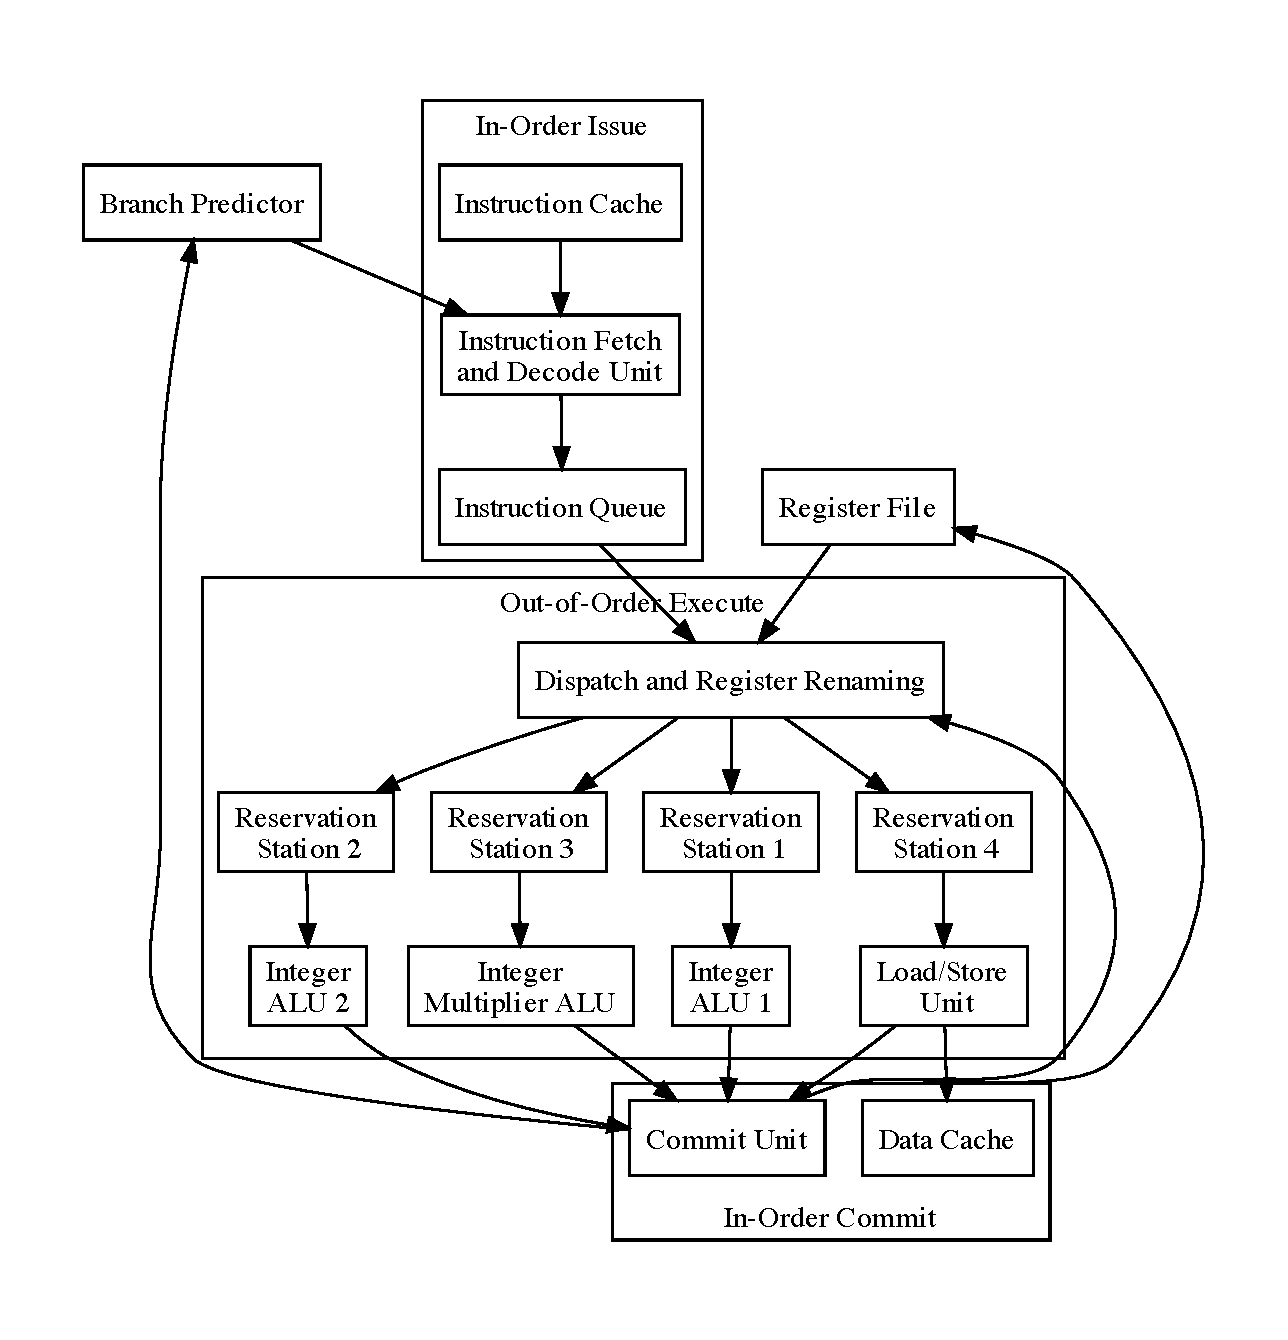
\includegraphics[width=\textwidth]{figures/design.pdf}
    \caption{System architecture using out-of-order execution and pipelined integer arthmetic. \label{fig:design}}
\end{figure}

\begin{figure}[h]
    \centering
    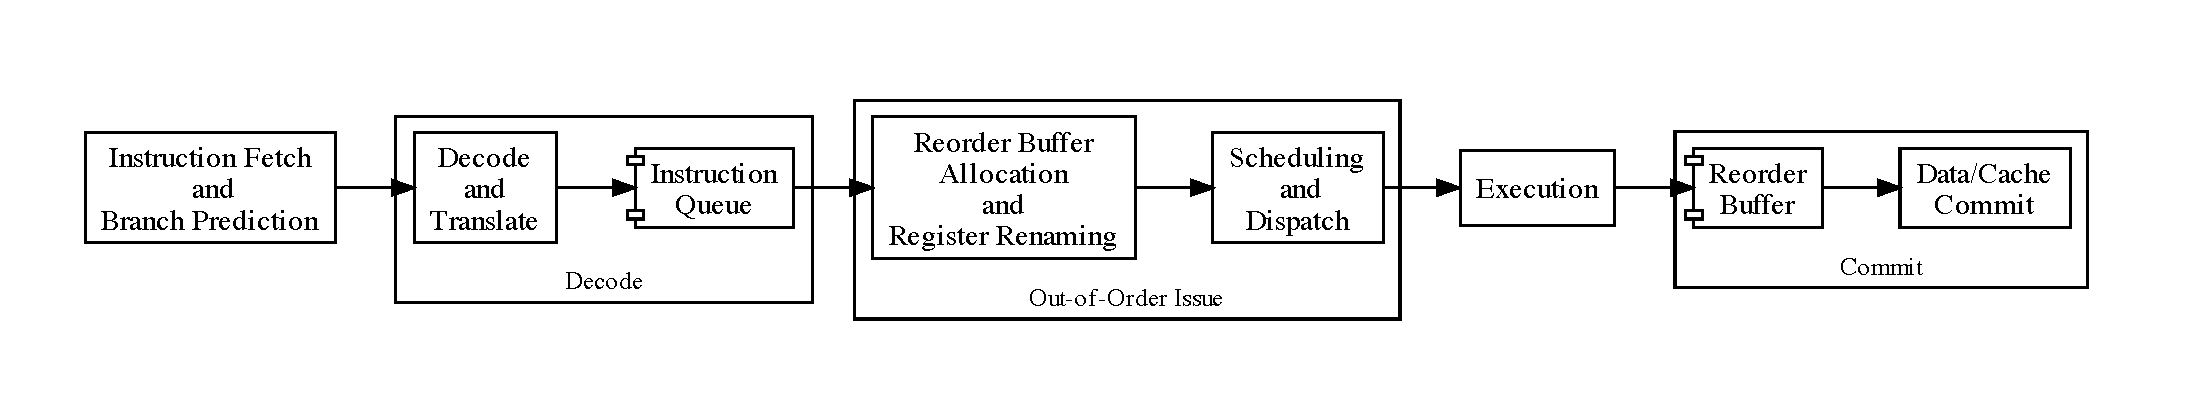
\includegraphics[width=1.1\textwidth]{figures/pipeline.pdf}
    \caption{Instruction pipeline. Pipeline stage is labeled in-box, unless superseded by an overbox. A component box indicates component (such as a FIFO) between stages. Not included in this diagram is the reservation stations and load/store buffer in the execution stage.\label{fig:pipeline}}
\end{figure}

The system design and instruction pipeline for our implementation is described
in Figure~\ref{fig:design} and~\ref{fig:pipeline}, respectively\footnote{This
diagrams borrow liberally from \emph{Computer Organization and Design: The 
Hardware/Software Interface} and \emph{Computer Architecture: A Quantitative 
Approach} by Hennessey and Patterson.}. The design extends our existing SMIPSv2 
implementation into three components: in-order instruction fetch and decoding, 
out-of-order execution units, and a commit unit. The instruction fetch and 
decode stage enqueues and dispatches instructions to reservation stations 
matching the appropriate execution unit, reordering as necessary to remove the 
pipelining hazards described in Section~\ref{sec:problem}. When the reservation 
station contains the appropriate operands for a given instruction, execution 
proceeds, and results are broadcast on a common data bus to waiting reservation 
stations and the branch prediction unit. The commit unit is implemented as a 
reorder buffer, and performs in-order commits to memory and the register file. 
Taken together with dispatch and register renaming, the reorder buffer and the 
reservation stations implement Tomasulo's algorithm.   

To introduce latency into our execution units, we will implement pipelined
integer arithmetic routines. With multiple integer arithmetic units, we will attempt
multiple-issue out-of-order execution using ALU instructions alone. We will also test
these pipelined integer units through standard unit testing, as in the audio pipeline
labs. 

We will use the existing SMIPS implementation and toolchain to provide inputs, gather 
outputs, log rule executions as traces, and benchmark our implementation. Verifying the 
correctness of the Tomasulo's algorithm implementation will first require modular refinement
of fundamental components, such as the reorder buffer and reservation stations, before 
they are incorporated into our existing SMIPS implementation. To verify functional 
correctness in instruction execution, we will unit test with short programs that 
emphasize particular issues: sequences of dependent instructions, sequences of independent
arithmetic instructions, small loops, atypical branch sequences, and memory operations. 
Verifying the traces for these smaller test programs will simplify execution debugging 
for the existing benchmarks. 


\subsection{FPGA Issues}

A working implementation of Tomasulo's algorithm on an FPGA is interesting because it would allow students and researchers to experiment with many processor microarchitectures. One
interesting experiment might be trying various numbers of ISA registers to find the fewest number of architectural registers that permits the same throughput. Another optimization
Tomasulo's algorithm enables is multiple dispatch. With the processor on an FPGA, different multiple dispatch schemes could be tested to determine what gives the best throughput.
Finally, an implementation of Tomasulo's algorithm could be used in a system that had special instructions with exceptional latencies. If one were to integrate an FFT instruction or
vector instructions, Tomasulo's algorithm would allow the implementor to see vastly improved performance with minimal effort.

Unfortunately, Tomasulo's algorithm makes heavy use of content-addressable memory (CAM). Although ASICs can easily incorporate CAM, FPGAs don't have built-in CAM, and so CAM
implementations can take many LUTs, leaving little space for additional hardware. Even a moderately large reorder buffer could take up too many LUTs to be synthesizable. Therefore
although we will try to optimize our design to fit on the FPGA, it may be impossible.

 \end{document}
